% Body of paper at ch4/papers/RLHF/main.tex
% Standalone preamble stripped; \input from the chapter wrapper.
\graphicspath{{ch4/papers/RLHF/}}





\section{Introduction}

Children do not learn language from exposure to input alone, but also through social interaction in which caregivers respond to their produced utterances \cite{fusaroli_caregiver_2023, masek_where_2021, clark_conversational_2020}. A long-standing question in language acquisition concerns the role of such feedback in shaping grammatical development, especially if caregiver responses can  help the learner know when their productions were well- or ill-formed \cite[see review in][]{, sokolov_changing_1994}. 

Although caregivers rarely provide explicit correction of grammatical errors \cite{brown_derivational_1970}, researchers have proposed that they nevertheless provide global, noisy feedback from which children can infer whether their utterances were likely grammatical or ungrammatical \cite[e.g.,][]{hirsh-pasek_brown_1984, demetras_feedback_1986, sokolov_changing_1994}. In this view, the child can be understood as learning in a reinforcement-like fashion, using the valence of the feedback as positive or negative rewards that guide which productions to maintain or adjust in future interactions \cite[e.g., see][]{whitehurst_what_1988, nikolaus_communicative_2023}.

The developmental literature has documented several forms of caregiver response that can be interpreted, within a reinforcement-learning framework, as valenced feedback. The most direct examples are \textit{communicative feedback} cues, namely a) acknowledgments (e.g., "okay", "yeah"), which signal communicative success and thus increase the likelihood that the child's sentence was well-formed, and b) clarification requests (e.g., "huh?", "what?"), which signal communicative failure or misunderstanding and thus increase the likelihood that the sentence was ill-formed \cite{clark_conversational_2020, demetras_feedback_1986, newport_mother_1977, saxton_prompt_2005}.  A second relevant class is \textit{semantic contingency}, or the extent to which caregiver responses remain responsive to the child's topic and intended meaning  \cite{hoff-ginsberg_topic_1987, che2018assessing, hirsh2015contribution}. The degree of this contingency captures the feedback valence: low contingency in the caregiver response signals semantic misalignment and thus increases the likelihood that the child’s utterance was ill-formed.

There are other forms of caregiver feedback that also provide such valenced signals, even if they have not traditionally been associated with this learning framework. Perhaps most directly relevant to grammar learning is \textit{structural alignment} \cite{fusaroli_caregiver_2023, dale_unraveling_2006, fernandez_quantifying_2014}, whereby caregivers respond by reusing the child's syntactic frame while potentially introducing different lexical content (e.g., child: “I eat” (Subject-Verb) → caregiver: “Mommy eats too”). Here, the feedback valence is reflected in whether such alignment occurs, signaling support for the child’s use of that syntactic frame. A final type of feedback is \textit{affective feedback}, such as whether caregivers respond with positive affect (e.g., "that's amazing!") versus a more emotionally neutral response \cite{rivero2023relations}.
 
These cues are far more available to children than explicit grammatical corrections, making their role in language learning much more plausible \cite{demetras_feedback_1986, hirsh-pasek_brown_1984}. Yet, they provide only indirect and noisy learning signals. First, they are not always directed at grammar. Second, even when grammar is relevant, the signal is global (i.e., utterance-level) and does not identify the specific error within the utterance. This makes \textit{credit assignment} a central challenge \cite{marcus_negative_1993, pinker_learnability_1989, saxton_contrast_1997}, and also makes interactive learning from caregiver feedback an interesting empirical case.

Nevertheless, little is known about how these different feedback types contribute to children’s grammatical learning. 
%This is due, at least in part, to limitations of traditional methods. Laboratory experiments make it possible to test the child's ability to learn from feedback, but they lack ecological validity. 
While corpus studies allow a quantitative account of caregivers' feedback behavior, \textit{the causal effect} of each type of feedback or reward on learning remains difficult to establish. A common methodological issue facing previous attempts \cite[e.g., see discussion in][]{saxton_negative_2005} is that different types of feedback are provided to the same child, making it difficult---and ethically problematic---to isolate their effect over the developmental timescales on which language is learned.

%for learning about the gra  including through clarification requests, repetitions, and reformulations \cite{hirsh-pasek_brown_1984, demetras_feedback_1986, saxton_negative_2000, chouinard_adult_2003, nikolaus_communicative_2023a}. Yet caregiver feedback is not a single, uniform signal: caregivers also provide other contingent signals whose role in language learning remains poorly understood \cite{clark_conversational_2020, dingemanse_universal_2015}.


Recent computational work has begun to revisit these questions by using LMs as controlled learning environments for testing hypotheses about language learning, thereby combining the targeted precision of experimental methods with the ecological validity of corpus studies \cite[e.g.,][]{misra2024language}. Particularly relevant to our  question are studies that used Reinforcement Learning to investigate LMs' interactive learning strategies \cite{ma_babysit_2024, martins-etal-2025-upon, zhao-etal-2023-babystories, padovani2025dialogue, xu2025wanting}.

A closely related line of work has applied this approach to \textit{natural} child--caregiver interactions, using Reward Models trained from caregivers' feedback data. Language models are then fine-tuned using techniques inspired by Reinforcement Learning from Human Feedback \cite[RLHF,][]{ouyang_training_2022}. Available research using this approach has shown that some naturally occurring caregiver feedback, namely clarification requests, can improve the grammaticality of generated utterances \cite[e.g.,][]{nikolaus_fourtassi_2026}.
%More specifically, they pre-trained a language model on child-directed language and then fine-tuned it with PPO using a reward model trained to predict when caregivers produce clarification requests to children. 

%However, those improvements did not translate into gains on standard grammatical knowledge benchmarks such as Zorro and Blimp. 

\subsection*{The current study} 
Existing RLHF-based studies of caregiver naturally occurring feedback have focused primarily on clarification requests, leaving open whether other forms of social feedback have similar, weaker, or even negative effects on grammatical learning. The present study addresses this gap by comparing several theoretically motivated feedback types within the same controlled learning framework.

%covering some of the major proposals in the developmental literature, including communicative feedback (clarification requests and acknowledgements), semantic contingency, affective feedback, and structural alignment.  
%The paper is organized as follows: Section 2 describes the methodology; Section 4 presents results; and Section 5 discusses implications and limitations.

%At the same time, those improvements did not translate into gains on standard grammatical knowledge benchmarks, suggesting that clarification requests may not straightforwardly target all aspects of grammar, or that their function may not be reducible to grammatical correction alone. This raises a broader question: do different types of caregiver feedback shape different aspects of linguistic behavior, and if so, how can this be measured rigorously?


%The present paper extends prior work in two aspects. First, we move beyond clarification requests to  multiple types of communicative feedback, including acknowledgments and conversation alignment signals, each as a distinct reward signal in a reinforcement learning framework. This allows us to ask not only whether socially grounded feedback improves grammar learning, but also whether different feedback types produce qualitatively distinct effects. Second, we expand the evaluation framework beyond grammaticality scores to include generation-based metrics that assess the quality of model outputs in the context of child-caregiver interaction \cite{liu2024benchmarking}.


\section{Methods}  
\label{sec:methods}

Our method uses a two-stage learning setup designed to separate learning from linguistic exposure from learning driven by caregiver-feedback rewards.
%\footnote{Unless otherwise stated, and for reproducibility, we follow the original methodology and publicly available implementation as closely as possible.} 
In a first step, a small causal language model is pretrained on child-directed language (excluding children's production), providing an \emph{input-only} baseline that quantifies learning gains from linguistic exposure. In a second step, the model is fine-tuned via RL, using a reward model trained on the target caregiver's feedback valence. 
%This design allows us to test each reward type separately, thereby isolating their specific causal effects on learning independently of the other rewards.

%We adopt the LM + RLHF framework of \citet{nikolaus2026modelling}, by extending it from a single feedback signal (clarification requests) to four theoretically motivated reward types.

\noindent \textbf{Pre-training baselines}  We use a customized version of GPT-2 (2 layers, hidden size 512, 8 attention heads), pre-trained on CHILDES \citep{macwhinney2000childes}, using three pre-training scales (0.1M, 1M, and 10M words, see Appendix 4).

\noindent \textbf{Empirical Reward Models} For each feedback type, we trained reward models to capture naturally occurring patterns of caregiver feedback in child--caregiver interactions (using CHILDES dataset). Each reward model is trained to map children's utterances to a scalar, representing the valence of the target feedback (see Appendix 4). %Specifically, we fine-tuned a pre-trained DeBERTa model to predict the valence of the target feedback from children’s utterances. 
The valence values themselves were annotated prior to reward-model training using a range of automatic annotation tools (see below, and Appendix 3).

\noindent \textbf{Topline Reward Model}: we use an idealized reward that directly targets grammatical errors. This topline is not intended to produce empirically realistic results, but rather to serve as an upper bound on what grammatical learning is possible \textit{in principle} (see details in Appendix 4).
%assigns a scalar score to model-generated utterances according to the target feedback dimension. The reward models were based on DeBERTa-style classifiers for different feedback types. 

\noindent \textbf{RL fine-tuning} For each feedback/reward, the pre-trained models were fine-tuned using the corresponding reward models, using Proximal Policy Optimization \citep[PPO;][]{schulman_proximal_2017}. We included several safeguards to mitigate potential language drift (see Appendix 5).

\noindent \textbf{Training seeds and variability} To account for stochastic variability, we used, for each training scale, a fully crossed $3 \times 3 \times 3$ design over pretraining seeds, fine-tuning seeds, and generation seeds.

\begin{figure*}[t]
    \centering
    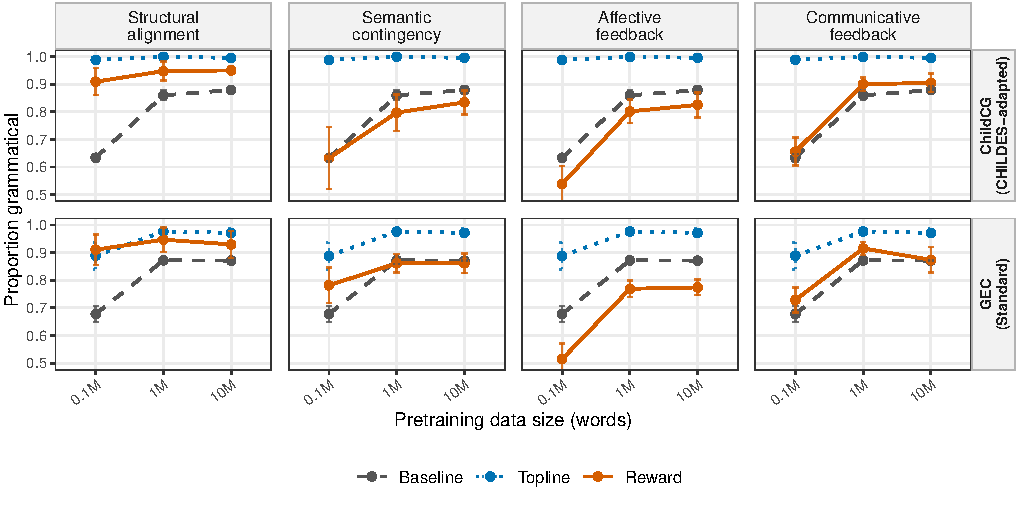
\includegraphics[width=\textwidth]{figures/figureC_generation_scale_trajectories.pdf}
    \caption{
    Generated-utterance grammaticality across pretraining scales for each reward.
    The top row shows results from the CHILDES-adapted ChildCG classifier, while the bottom row shows results using a standard GEC-based metric.
    Within each panel, baseline and topline trajectories are repeated to make the reward trajectory directly comparable.
    Means are computed over training seeds units after averaging over generation seeds. Error bars show $\pm 1$ standard deviation across training seeds.
    }
    \label{fig:generation_reward_scale}
\end{figure*}

\noindent \textbf{Annotation of the reward signals}  We considered the four classes of caregiver feedback mentioned in the introduction: communicative feedback, semantic contingency, structural alignment and affective feedback. For each type of feedback, we annotated the CHILDES child-caregiver conversations for the corresponding valence (See Appendix 3).
%\citep{nikolaus2023modeling,clark2018conversation}. 

% Each reward signal was designed to capture a different way in which caregivers may respond contingently to children’s utterances.


%\noindent \textbf{Structural alignment} Caregivers mirror the child's syntactic frame while potentially using different lexical content (e.g., child: \textit{``I eat''} $\to$ caregiver: \textit{``Mommy eats too''}). Following \citet{fernandez_quantifying_2014}, we quantified this as the proportion of Part-of-Speech bigrams produced by the child that were subsequently reused by the caregiver in the immediate response. 
%The target valence is this value.

%\noindent \textbf{Semantic contingency} This captures whether the caregiver response remains within the same conceptual or semantic topic (e.g., child: \textit{``lion''} $\to$ caregiver:
%\textit{``Yes, and a tiger!''}). We quantified this as the cosine similarity between sentence embeddings of child and adult turns, using a pre-trained BERT encoder. 
%The target valence is this value.

%\noindent \textbf{Affective feedback} This corresponds to when caregivers express positive affect  (e.g., \textit{``Yay, that's amazing!''}). We used a sentiment classifie \citep{liu2019roberta}r---it recognizes 6 categories; we select 3 that map to positive affects (warmth, sportiveness, and approval). 
%The target valence is are the values outputed by the classfier for each.

%We quantify this using a RoBERTa-based sentiment classifier\citep{liu2019roberta}.


\subsection{Evaluation}
\label{sec:eval}

We use two complementary evaluations that capture different aspects of grammatical behavior. 

\noindent  \textbf{Minimal-pair benchmarks}: we use Blimp \cite{warstadt2020blimp} and its CHILDES-adapted version Zorro \cite{huebner_babyberta_2021}. They test whether a model assigns higher probability to a grammatical sentence than to a minimally differing ungrammatical one. 
%\paragraph{Comprehension benchmarks} We evaluate models on BLiMP \citep{warstadt2020blimp} and Zorro \citep{huebner2021babyberta}, two minimal-pair benchmarks that test whether a model assigns higher probability to a grammatical sentence than to a minimally differing ungrammatical one. Following prior work\citep{nikolaus2026modelling}, we filtered out sentence pairs containing words that do not appear in the model’s training data. This evaluation measures whether reinforcement learning improves the model’s preference for grammatical over ungrammatical forms in controlled benchmark settings.

\noindent \textbf{Grammaticality of generated utterances} Free generations were scored using Child Conversational Grammaticality  \cite[ChildCG, ][]{nikolaus_automatic_2024}, a model adapted to CHILDES and its conversational context. In addition, we used a measure based on an off-the-shelf Grammatical Error Correction model \cite[e.g.,][]{rothe_simple_2021}. For each run and generation seed, we sampled up to 10,000 utterances using the Beginning-Of-Sentence (BOS) token as a prompt.

Both evaluation methods are broadly connected to child-language methodologies for evaluating grammatical development, which have included both controlled forced-choice tasks and analyses of children’s spontaneous and elicited productions \cite{ambridge2011child}.
%The results remained unchanged when using 100 samples per generation seed. This is the value we use.
%Although this model was not explicitly adapted to child-like language use or its conversational specificities, it provides a complementary metric based on more general grammatical error detection.
%For each model, we sampled 10,000 utterances using the beginning-of-sentence token as a prompt. We then scored these generations using two automatic grammaticality measures: a grammatical error correction-based model and a grammaticality annotation model fine-tuned on child-caregiver data. This generation-based evaluation is important because prior work found that feedback may improve the grammaticality of model productions even when it does not improve performance on grammatical minimal-pair benchmarks.
%\textbf{Additional analyses} We also evaluate the model generation in term of utterance length, lexical entropy, rate of non-words, function-word density. %following \citet{liu2024benchmarking}. 
%These metrics reveal whether differences in grammaticality co-vary with broader changes in production style (e.g., longer outputs accruing more errors, or reduced function-word use signalling grammatical impoverishment).





\section{Results}
\label{sec:results}

First, we compared the baseline models, trained only on linguistic input, with the same models further fine-tuned using the grammar topline reward model (Figure \ref{fig:topline} in Appendix). The topline improves both minimal-pair benchmark performance and the grammaticality of generation, showing the current framework can, in principle, lead to \textit{grammatical} learning above and beyond pre-training. 
%However, gains on the Zorro and BLiMP benchmarks remain relatively small compared to generated-utterance grammaticality.

Moving to the empirical reward models, we found no consistent improvement on the minimal-pair benchmarks (Figure~\ref{fig:benchmark_reward_scale} in Appendix). Across Zorro and BLiMP, none of the reward types reliably improved over the baseline. This echoes a broader pattern in recent studies showing
that interactive strategies  struggle to improve performance on these benchmarks (see also Limitations). In contrast, the generation results showed measurable effects on grammaticality (Figure \ref{fig:generation_reward_scale}). Across both ChildCG and GEC, the overall trends were largely consistent. Structural alignment produced the strongest and most consistent improvement across scales and metrics. Communicative feedback showed an overall positive effect, especially under ChildCG, but the gains were smaller. In contrast, semantic contingency and affective feedback generally reduced grammaticality below the baseline. 

Regarding the effect of pre-training size, the low-resource condition at 0.1M was visibly noisier, with larger variability across runs, excessively high non-word rates (Figure ~\ref{fig:covariates_reward_scale} in Appendix, bottom row), and overall low grammaticality scores. The effects became much more consistent from 1M words onward,
suggesting that a minimum amount of pre-training data is needed before reward-specific effects can emerge robustly.

We tested these qualitative patterns statistically using a mixed-effect logistic model. Predictors included reward type, pretraining scale, and their interaction. We additionally added the following predictors as controls \uline{a) utterance length}, since longer utterances may naturally provide more opportunities for errors, and \uline{b) rate of non-words generated}, since out-of-dictionary forms may be penalized by grammaticality classifiers for reasons that are not strictly grammatical.  Finally, we included a random intercept for generation run to account for the fact that sampled utterances from the same seeds are not independent.


\begin{table}[t]
\centering
\small
\begin{tabular}{lll}
\toprule
Reward family & 1M & 10M \\
\midrule
Structural alignment      & $+.077^{***}$ & $+.060^{***}$ \\
Semantic contingency      & $-.092^{***}$ & $-.061^{***}$ \\
Affective feedback        & $-.038^{*}$   & $-.031^{*}$   \\
Communicative feedback    & $+.033^{*}$   & $+.024^{\dagger}$ \\
\quad Acknowledgement     & $+.017$       & $+.017$       \\
\quad Clarification request  & $+.050^{***}$ & $+.031^{*}$   \\
\bottomrule
\end{tabular}
\caption{
Model-estimated change in grammaticality probability relative to baseline, using the ChildCG metric at the 1M and 10M pretraining scales.
$\dagger p<.10$, $^{*}p<.05$, $^{**}p<.01$, $^{***}p<.001$.
}
\label{tab:grammar_reward_effects}
\end{table}

Table~\ref{tab:grammar_reward_effects} reports model-estimated changes in grammaticality probability relative to the baseline, using the more robust pretraining scales (1M and 10M). Mirroring the pattern in Figure~\ref{fig:generation_reward_scale}, structural alignment showed the clearest improvement. In contrast, semantic contingency and affective feedback both reduced grammaticality. Communicative feedback improved grammaticality at 1M and showed a marginally significant positive effect at 10M. When communicative feedback was split into its two components, only clarification requests showed a significant effect, whereas the acknowledgment-based reward model did not.


%Regarding our control variables, and as expected, utterance length was itself associated with grammaticality: longer utterances were \textit{less} likely to be judged grammatical (Odd Ratio = 0.84, $p < .001$). Crucially, however, this does not explain away the reward effects reported in Table \ref{tab:grammar_reward_effects}; as the estimated reward effects correspond to differences in grammaticality \textit{after} controlling for length. As for our second control variable:  non-word rate, it did not reliably predict lower grammaticality (OR = 1.02, $p = .063$).

\section{Discussion and Conclusions}

We investigated which forms of caregiver feedback support LMs' grammaticality within an RLHF-inspired framework. We isolated and compared major feedback types, providing insight into their specific effects and relative contributions.

The main finding was that Structural Alignment systematically improves grammaticality. While previous work found correlational evidence to this link \cite{fusaroli_caregiver_2023}, the current result demonstrates, at scale, a novel and plausible \textit{mechanistic} account: Caregiver's structural alignment can support grammar learning \textit{because} this reinforces the child's use of structures that are grammatical---caregivers naturally tend to (re-)use grammatical sequences more often than ungrammatical ones.
%This mechanistic insight is promising, but it should be examined further in future dedicated work so as to fully characterize its conrtibuti on our understanding of alignment in language development. 
%By comparing multiple reward types within the same framework, we were able to put the effect of communicative feedback into perspective. 
Communicative Feedback also improved grammaticality, though to a lesser extent. The improvement is consistent with prior work, especially on clarification requests \cite{nikolaus_fourtassi_2026, clark_conversational_2020}. 
%However, by comparison, its effect was smaller than that of structural alignment. %and was not uniform across its two components: clarification requests and acknowledgements.

As for Semantic Contingency and Affective Feedback, they  \textit{reduced} grammaticality. We did not anticipate this outcome; however, it can be understood in the broader context of development.
%This should not be interpreted as evidence that these rewards are unimportant for development. Rather, it suggests that different 
Based on the supplementary analyses in Figure \ref{fig:covariates_reward_scale}, and models' generation samples in Table \ref{tab:sampled_childcg_examples} (Appendix), Affective Feedback increased utterance length, suggesting a role in eliciting
longer vocalization \cite[see also][]{goldstein2003social}. Semantic Contingency increased the use of content words and preserved greater lexical diversity, in line with findings in lexical development \cite{che2018assessing}.
%Thus, semantic contingency and affective feedback may support important dimensions of language and socio-cognitive development, without being ideally conducive to grammar learning specifically. 

To conclude, different types of feedback push generation in different directions: some improve grammaticality, while others encourage other properties of language learning and use. 
%Although we focused on grammar, this is only one dimension of development. Rewards such as semantic contingency and affective feedback may be less useful for grammar directly, but still important for semantic coherence, engagement, pragmatic appropriateness, lexical development, or children’s willingness to participate in interaction. 
Future work should adopt a broader framework, investigating how these feedback types may support \textit{complementary} aspects of language learning beyond grammar.

\subsection*{Limitations}

A limitation of our study is that the effects of the empirical rewards were observed in model generation, but not in minimal-pair benchmarks. This echoes a broader pattern in recent studies showing that interactive strategies generally struggle to improve performance on minimal-pair benchmarks of grammar such as BLIMP and Zorro \cite{zhao-etal-2023-babystories, padovani2025dialogue, nikolaus_fourtassi_2026, stopler2025towards}.

This raises an important theoretical question: To what extent does grammaticality in generation reflect grammatical knowledge? 
%This question echoes a broader distinction in both child language research and formal language learnability: producing well-formed utterances does not necessarily equate to acquiring grammatical knowledge that generalizes. In child language research, this issue appears in debates about productivity and overgeneralization (Ambdige). In formal learnability, recent work distinguishes the ability to generate valid strings from the stronger problem of identifying the underlying language (Kleinberg and Mullainathan, 2024). We do not attempt to address this broad issue here.
This remains a debated question in child language research \cite{ambridge2011child, chater2018language};
%and formal language learnability \cite{kleinberg2024language} 
and we do not aim to address this general question here.


In the specific case of the present study, however, it is cautious to interpret the generation-based results more narrowly: they test how reward fine-tuning changes the model’s productive behavior; they do not directly test whether the model has acquired grammatical knowledge that can generalize. 
Note that even under this conservative interpretation, the generation-based results remain informative for theories of language development. Unlike traditional corpus-level correlations, the rewards here were used as interventions within a computational learning system, allowing us to test whether optimizing for these signals \textit{causally} shifts the model’s production policy in grammar-relevant directions.

%higher generated grammaticality does not by itself demonstrate the acquisition of general grammatical knowledge.
Nevertheless, a model that becomes more grammatical in free generation does not necessarily mean it has learned grammatical regularities that generalize beyond the specific utterance types favored during fine-tuning.
%across lexical items and sentence constructions.
Minimal-pair benchmarks---though not perfect \cite{martinez2023evaluating}---are useful precisely because they intend to test this stronger criterion for learning. Our null results on BLiMP/Zorro (Figure \ref{fig:benchmark_reward_scale}) therefore matter. They suggest that the empirical rewards did not produce grammatical generalization---at least, not of the kind captured by these benchmarks.

That said, while this conclusion may be partly correct, it would be premature to draw it too strongly here without further research. Existing minimal-pair benchmarks do not exhaust the space of possible grammatical generalizations. In particular, even child-adapted benchmarks such as Zorro primarily target classic grammatical phenomena, but do not directly target some of the errors that are especially common in child language \textit{production} and may therefore also be reproduced in our generated data---including missing subjects, objects, auxiliaries, or determiners, among others \cite{saxton2005prompt, hiller_data-driven_2016, nikolaus_automatic_2024}. This is important because, in an RL fine-tuning setting,  errors that are sampled in the model's productions are the ones that receive direct corrective pressure from the reward signal.

Another concern is that reward fine-tuning may narrow the model’s production distribution, reducing diversity and potentially harming generalization. However, while this may be partly true, some narrowing may still be compatible with grammatical learning, and perhaps even expected if the model moves away from noisy or ill-formed productions. For instance, in our analyses, the grammar topline was relatively the least lexically diverse condition (Figure~\ref{fig:covariates_reward_scale}, Lexical Entropy, Appendix), yet it produced the clearest gains on the minimal-pair benchmarks (Figure~\ref{fig:topline}, Appendix). Thus, reduced lexical diversity does not in itself prevent grammatical generalization. The more central question is whether reward-induced changes target grammatical phenomena that can generalize beyond the sampled utterances themselves.

Testing this stronger learning claim, thus, remains an important direction for future work. It requires conducting large scale corpus exploration of the grammatical errors found in both child and model productions, and to use these bottom-up insights to build targeted tests around the relevant phenomena. This would help determine whether the reward-induced gains observed here reflect merely local shifts in surface production patterns or more abstract grammatical generalizations.

%Such errors account for a large share of children’s grammatical errors 

%To sum up, while this work shows that caregiver-derived rewards can shape production in grammar-relevant ways, it does not yet establish generalized grammatical learning.



%To avoid misunderstanding, the concern is not simply that reward fine-tuning narrows the model’s production distribution. Some narrowing may be compatible with grammatical learning, and perhaps even expected if the model moves away from noisy or ill-formed productions. For instane, in our analyses, the grammar topline was relatively the least lexically diverse condition (Figure~\ref{fig:covariates_reward_scale}), yet it produced the clearest gains on the minimal-pair benchmarks (Figure~\ref{fig:baseline_topline_scale}). Thus, reduced lexical diversity does not in itself prevent grammatical generalization. The more central question is whether reward-induced changes target grammatical phenomena that transfer beyond the sampled utterances themselves.


%The modest benchmark gains obtained with the grammar topline (Figure \ref{fig:baseline_topline_scale}) further support this interpretation. Even when the reward has direct access to grammaticality supervision, the baseline model is updated only through feedback on its \textit{own generated productions}. If these productions rarely contain the kinds of grammatical errors represented in BLiMP/Zorro, then even an idealized grammar reward has few opportunities to penalize those errors and reinforce the corresponding grammatical alternatives. Reward fine-tuning may therefore improve generated grammaticality while producing only modest gains on minimal-pair benchmarks.



\section*{Ethical considerations}

This work uses existing child-caregiver corpora and does not involve new data collection. Because the data involve children, we treat the corpora as sensitive and report only aggregate model-level results, without attempting to identify individual children, caregivers, or families. The proposed modeling framework is intended as a tool for studying hypotheses about language development, not for evaluating individual children or caregivers.

%The fact that even the idealized grammar topline---trained specifcially to capture the errors covered in Blimp and Zorro---produced only modest benchmark gains further suggests that children/models may only produce a small subset of the errors that are covered in the benchmarks. 
%We reported results using evaluation of model generation. The minimal-pair benchmarks were not sensitive enough to detect the effects of our empirically derived rewards--- although, to be sure, they did capture the effects of the idealized topline reward, suggesting possibility for improvement in principle. This contrast echoes a broader pattern in recent work reporting very limited effects of interactive learning strategies on minimal-pair grammatical benchmarks (e.g., Francesca/Biazza etc.), with studies focusing on evaluating model generation producing the most promising results (Lisa Ho)

%Work on RLHF for chatbots provides a useful but only partial analogy. Reward fine-tuning often produces clear changes in generated behavior, while its effects on fixed benchmark datasets can be weaker (Ouygang et al., 2022). However, our case is more specific. We are not comparing a change in one aspect of generation, such as helpfulness or style, with benchmarks targeting a different ability, such as reasoning. Both our generation-based evaluation and our minimal-pair benchmarks are intended to assess grammaticality. The divergence between them is therefore non-trivial: under a broad interpretation of grammatical knowledge, one might expect improvements in generated grammaticality to be accompanied by improvements on controlled grammatical contrasts.


-









\iffalse
We report results in three steps. First, we examine benchmark-based grammaticality on BLiMP and Zorro. Second, we evaluate the grammaticality of model-generated utterances. Third, we analyze additional properties of the generated outputs to better understand why reward conditions differ.


\subsection{Benchmark-based grammaticality}
\label{sec:results_benchmark}

Across all four caregiver-derived reward conditions, RL fine-tuning yields little to no improvement over the input-only baseline on BLiMP and Zorro (Figure~\ref{fig:blimp}--\ref{fig:zorro}). The pattern holds regardless of training data size.

% Reinforcement learning with caregiver-derived rewards yields little to no improvement over the input-only baseline on BLiMP and Zorro. This is true for all reward types tested: communicative feedback, structural alignment, semantic contingency, and affective feedback. 

This replicates the finding of \citet{nikolaus2026modelling} for communicative feedback and generalises it to structural alignment, semantic contingency, and affective feedback: none of the feedback signals tested here systematically improves performance on grammatical minimal-pair benchmarks.

% This result replicates the benchmark-based pattern reported by Nikolaus and Fourtassi (2025): reinforcement learning from communicative feedback does not straightforwardly improve performance on standard grammaticality benchmarks. More generally, our results suggest that caregiver-derived rewards considered here do not strongly improve the type of grammatical preference measured by BLiMP and Zorro. 

The grammar topline, which directly rewards grammaticality, does improve benchmark performance, confirming that the RL framework is capable of driving benchmark gains when the reward explicitly targets them. The failure of caregiver-derived rewards on benchmarks, therefore, reflects the indirect nature of these signals, not a limitation of the learning procedure.

% The artificial grammar topline, which directly rewards grammaticality, shows that this limitation is not due to the RL framework itself, but to the indirect nature of caregiver-derived feedback signals. 



\begin{figure*}[ht]
\includegraphics[width=1\textwidth]{1e06_reward_group_se_best_zorro.png}
\caption{Results of zorro evaluation for baseline (input-based training only) and fine-tuned models (input-based training and feedback-based training). 
Asterisks indicate significant differences in scores for baseline versus fine-tuned models as measured using a two-sided t‐test: *p < 0.05; **p < 0.01; ***p < 0.001. M, million.}
\label{fig:zorro}
\end{figure*}


\begin{figure*}[ht]
\includegraphics[width=1\textwidth]{1e06_reward_group_se_best_blimp.png}
\caption{Results of blimp evaluation for baseline (input-based training only) and fine-tuned models (input-based training and feedback-based training). 
Asterisks indicate significant differences in scores for baseline versus fine-tuned models as measured using a two-sided t‐test: *p < 0.05; **p < 0.01; ***p < 0.001. M, million.}
\label{fig:blimp}
\end{figure*}

\subsection{Generation-based grammaticality}
\label{sec:results_generation}

In contrast to the benchmark results, generation-based evaluations reveal clearer differences between reward types (Figures~\ref{fig:childes}--\ref{fig:gec}). 

Structural alignment produces the strongest improvement in grammaticality, with gains on both generation-based measures. This suggests that caregiver responses which mirror or extend the child's syntactic structure may provide a particularly useful signal for improving grammatical production. 

Communicative feedback also improves generation-based grammaticality, although more moderately than structural alignment. This partially replicates prior findings on clarification requests \citep{nikolaus2026modelling}, while suggesting that repair-oriented feedback may not be the only caregiver signal relevant to grammatical development. At the same time, communicative feedback may not be exclusively grammatical in function: clarification requests and acknowledgments could also reflect broader issues of intelligibility, attention, discourse coordination, or communicative success.

semantic contingency and affective feedback, by contrast, do not improve generated grammaticality; depending on training size and evaluation measure, they have little or even a detrimental effect. This is notable because these feedback types are central to child-caregiver interaction yet neither benefits grammatical production in our model.

% but it suggests that their primary contribution may not be grammar-specific. 

\begin{figure*}[ht]
\includegraphics[width=1\textwidth]{latex/1e06_reward_group_se_grammaticality_childes.png}
\caption{Results of childes evaluation for baseline (input-based training only) and fine-tuned models (input-based training and feedback-based training). 
Asterisks indicate significant differences in scores for baseline versus fine-tuned models as measured using a two-sided t‐test: *p < 0.05; **p < 0.01; ***p < 0.001. M, million.}
\label{fig:childes}
\end{figure*}


\begin{figure*}[ht]
\includegraphics[width=1\textwidth]{latex/1e06_reward_group_se_grammaticality_gec.png}
\caption{Results of gec evaluation for baseline (input-based training only) and fine-tuned models (input-based training and feedback-based training). 
Asterisks indicate significant differences in scores for baseline versus fine-tuned models as measured using a two-sided t‐test: *p < 0.05; **p < 0.01; ***p < 0.001. M, million.}
\label{fig:gec}
\end{figure*}

\subsection{Additional analyses of generated utterances}

To understand the production findings, we analyse three additional
properties of the generated utterances, following
\citet{liu2025benchmarking}: utterance length, lexical entropy,
and function-word density (Figure~\ref{fig:length}--\ref{fig:funcden}).

% The additional generation metrics help us clarify why some reward conditions could improve grammaticality while others do not. 

\paragraph{Utterance length}
affective feedback produces the longest utterances across training
conditions. Longer outputs create more opportunities for grammatical errors,
which provides a partial account of the detrimental effect observed for this reward. Crucially, however, semantic contingency also performs poorly on grammaticality despite producing utterances that are slightly \emph{shorter} than the baseline, not longer. Length is therefore not a sufficient explanation for the null and negative effects, and the remaining analyses are needed to complete
the picture.

% affective feedback produces longer utterances, which may partly explain its weaker grammaticality performance: longer outputs create more opportunities for grammatical errors. However, length alone cannot explain all of the results. semantic contingency also performs poorly on grammaticality, even though its outputs are not especially long. 

\paragraph{Lexical entropy}
Both semantic contingency and affective feedback produce higher lexical entropy than the baseline and than the other reward conditions, indicating that these rewards encourage more diverse, less predictable word choices. High lexical diversity may serve communicative functions, thus enriching the semantic and expressive range of utterances, but it also reduces the model's tendency to rely on the high-frequency, grammatically stable patterns that support well-formed productions.

% Lexical entropy is higher for both semantic contingency and affective feedback (especially compared to the topline), suggesting that these rewards encourage more diverse outputs. Such diversity may be useful for exploration or communicative richness, but it may also make grammatical control more difficult. 

\paragraph{Function-word density}
Finally, all caregiver-derived rewards reduce function-word density relative to the baseline, with the strongest reduction under semantic contingency. Since function words carry much of the grammatical scaffolding of an utterance, this reduction may help explain why some rewards push the model toward content-rich but less grammatically stable productions. 


\begin{figure*}[ht]
\includegraphics[width=1\textwidth]{latex/1e06_reward_group_se_sent_len_mean.png}
\caption{Results of gec evaluation for baseline (input-based training only) and fine-tuned models (input-based training and feedback-based training). 
Asterisks indicate significant differences in scores for baseline versus fine-tuned models as measured using a two-sided t‐test: *p < 0.05; **p < 0.01; ***p < 0.001. M, million.}
label{fig:gec}
\end{figure*}

\begin{figure*}[ht]
\includegraphics[width=1\textwidth]{latex/1e06_reward_group_se_entropy_reg.png}
\caption{Results of gec evaluation for baseline (input-based training only) and fine-tuned models (input-based training and feedback-based training). 
Asterisks indicate significant differences in scores for baseline versus fine-tuned models as measured using a two-sided t‐test: *p < 0.05; **p < 0.01; ***p < 0.001. M, million.}
label{fig:gec}
\end{figure*}

\begin{figure*}[ht]
\includegraphics[width=1\textwidth]{latex/1e06_reward_group_se_func_den_mean.png}
\caption{Results of gec evaluation for baseline (input-based training only) and fine-tuned models (input-based training and feedback-based training). 
Asterisks indicate significant differences in scores for baseline versus fine-tuned models as measured using a two-sided t‐test: *p < 0.05; **p < 0.01; ***p < 0.001. M, million.}
label{fig:gec}
\end{figure*}





\section{Discussion}
Our results support a differentiated view of caregiver feedback in grammatical development. Caregiver-derived rewards do not behave like a single generic signal for grammatical improvement: their effects depend on the type of feedback modeled and on the evaluation used. In particular, we find little to no improvement on minimal-pair benchmarks, but clearer effects on the grammaticality of generated utterances, suggesting that feedback-based reinforcement learning affects production more than benchmark-based grammatical preferences.

Structural alignment provides the strongest improvement in generated grammaticality. This suggests that caregiver responses which mirror or extend the child's syntactic structure may provide a useful signal for grammar learning, possibly because they preserve aspects of linguistic form and expose the learner to reusable grammatical frames. Communicative feedback also plays a role in grammaticality, but the effect is more limited. This may be because clarification requests and acknowledgments are informative but noisy: they can reflect grammatical problems, but also intelligibility, attention, ambiguity, or broader communicative success.

By contrast, semantic contingency and affective feedback do not improve grammaticality, and may even reduce it. This should not be taken to mean that they are developmentally uninimportant. Rather, their main role may lie outside grammar : semantic contingency may support semantic coherence and common ground, while affective feedback may encourage participation and vocalization. This interpretation seems to be supported by our additional analyses. 

More broadly, our approach shows how computational modeling can be used to isolate feedback signals that are normally intertwined in natural child-caregiver interaction. This makes it possible to test the causal effects of different forms of feedback in a way that would be difficult, if not impossible, in studies with children. In this sense, the present work contributes to theories of language development in and through social interaction by asking not only whether feedback matters, but which feedback matters for which aspect of learning. 

Several limitations remain. First, our analyses aggregate children across a wide age range, from toddlers to older children. This may obscure developmental differences in the function of caregiver feedback: caregivers may encourage younger children to vocalize and participate regardless of grammatical accuracy, while older, more fluent children may receive feedback that is more closely tied to grammatical form. Second, we test feedback in isolation, whereas natural caregiver responses often combine several signals at once. Future work therefore aim to model combinations of rewards, provided that their relative weights can be estimated from natural interaction. More generally, future evaluations should extend beyond grammar to include semantic coherence, conversational relevance, lexical development, pragmatics and willingness to produce language, ideally using multimodal and longitudinal data. 




\section{Conclusion}

Overall, our results show that caregiver-derived rewards do not have uniform effects on grammaticality. Minimal-pair benchmarks showed little improvement across empirical rewards, whereas generation-based evaluations revealed clearer differences. Structural alignment produced the strongest grammaticality gains, communicative feedback yielded more moderate improvements, and semantic contingency and affective feedback did not improve grammaticality in this setup. Additional analyses showed that these rewards also shaped broader properties of the generated utterances, including length, lexical entropy, function-word density, and question rate.

These findings suggest that caregiver feedback should not be treated as a single, generic learning signal. Different rewards push generation in different directions: some make utterances more grammatical, while others encourage different properties of language use. Here, we focused primarily on grammaticality, but this is only one dimension of language development. Rewards such as semantic contingency and affective feedback may be less useful for improving grammar directly, while still being important for other aspects of learning, such as semantic coherence, conversational engagement, pragmatic appropriateness, lexical development, or children’s willingness to participate in interaction. Future work should therefore evaluate caregiver-derived rewards in a broader developmental framework, where different feedback signals may support different, complementary aspects of language learning.

Overall, the results show that caregiver-derived rewards do not have uniform effects on grammaticality. While benchmark-based evaluations show little improvement across rewards, generation-based evaluations reveal clearer differences: structural alignment provides the strongest gains, communicative feedback yields more moderate improvements, and semantic contingency and affective feedback do not improve grammaticality. The additional analyses further show that these rewards also affect broader properties of model output, including length, entropy, and function-word density.


\fi




\clearpage
\twocolumn[{
\section*{Appendix 1: Supplementary Analyses}
\label{app:analyses}

\begin{center}
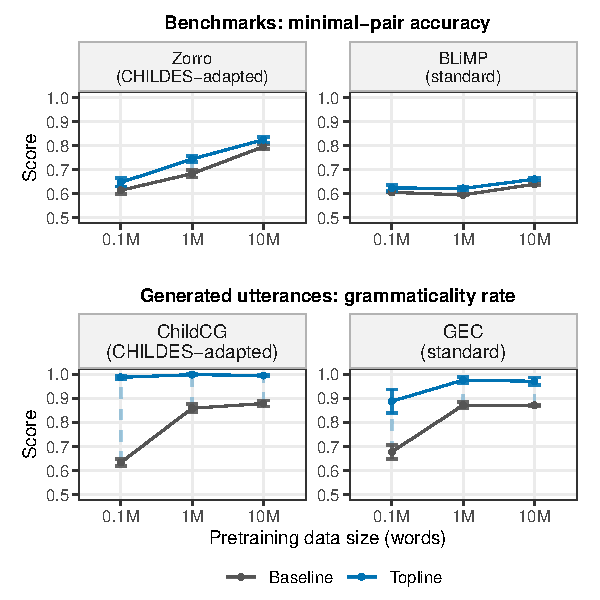
\includegraphics[width=0.7\textwidth]{figures/figureA_baseline_topline_scale_mixed_sources_new.pdf}

\captionof{figure}{
Baseline and Topline performance across pretraining scales. The top row reports minimal-pair benchmark accuracy for Zorro and BLiMP. The bottom row reports grammaticality of generated utterances, using the ChildCG or GEC-based metric. Points show means across trainings seeds (after averaging over generation seeds). Error bars show ±1 standard deviation across these independent units.
}
\label{fig:topline}
\end{center}
}]

\begin{figure*}[t]
    \centering
    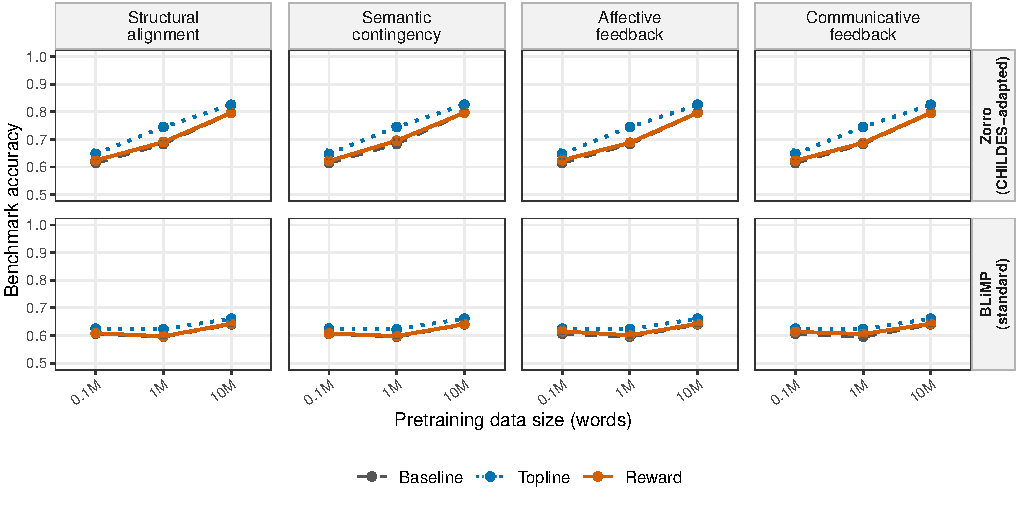
\includegraphics[width=\textwidth]{figures/figureB_benchmark_scale_trajectories.pdf}
    \caption{
    Benchmark performance across pretraining scales for each reward family.
    Rows show Zorro and BLiMP minimal-pair accuracy; columns show the four empirical reward families.
    Within each panel, the baseline and topline trajectories are repeated to make the reward trajectory directly comparable at each scale.
    Means are computed over training seeds, after averaging over generation seeds. Error bars show $\pm 1$ standard deviation across independent units.
    }
    \label{fig:benchmark_reward_scale}
\end{figure*}


\begin{figure*}[t]
    \centering
    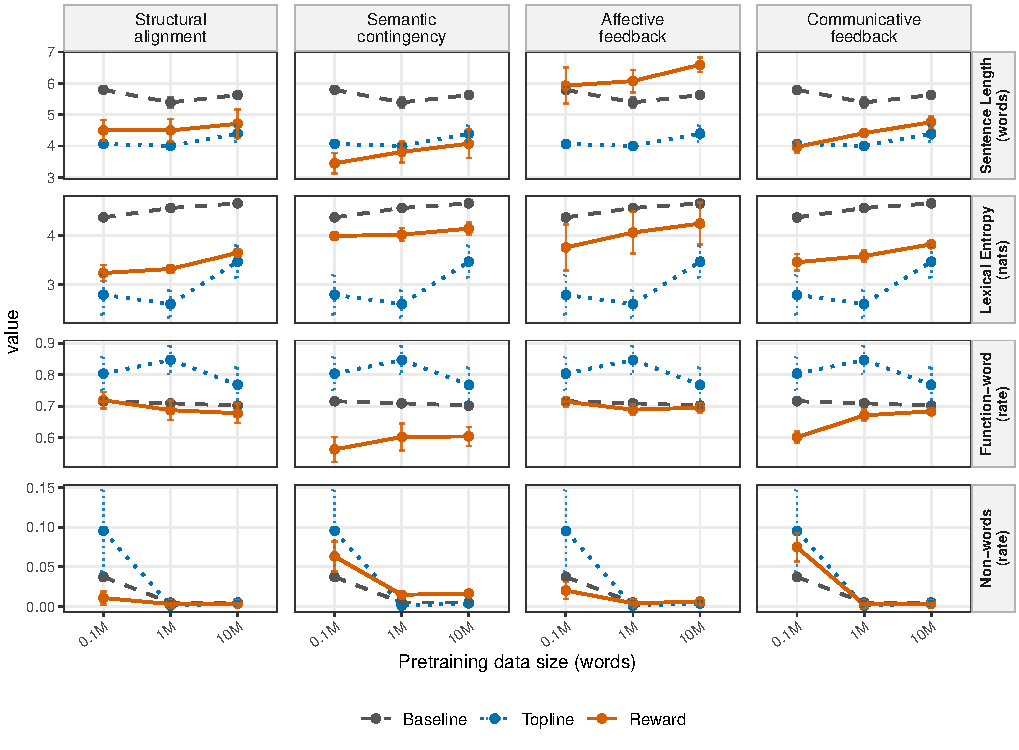
\includegraphics[width=\textwidth]{figures/figureD_covariates_scale_trajectories.pdf}
    \caption{
    Properties of generated utterances: Sentence length, pooled lexical entropy, function-word density, and rate of non-words.
    Points show means for each reward across training seeds, with error bars indicating $\pm 1$ standard deviation across these seeds.
    Within each panel, baseline and topline trajectories are repeated to make the reward trajectory directly comparable at each scale.
    }
    \label{fig:covariates_reward_scale}
\end{figure*}

\clearpage


\begin{table*}[t]
\section*{Appendix 2: Examples of Model-Generated Utterances}
\vspace{1em}
\centering
\scriptsize
\setlength{\tabcolsep}{3.5pt}
\renewcommand{\arraystretch}{1.18}

\begin{tabular}{
p{0.12\textwidth}
p{0.12\textwidth}
p{0.30\textwidth}
>{\columncolor{gray!15}}p{0.38\textwidth}
}
\toprule
Reward type &  & ChildCG = 1 (grammatical) & ChildCG = 0 (ungrammatical) \\
\midrule

\textbf{Baseline} &  &


\textit{you want to look at some more pictures?}

\textit{oh, is that what it looks like?}

\textit{it is a big boy now isn't it?}

\textit{have you not any other little boys?}
&
\textit{this piece of cake?}

\textit{because you can see mummy's poorly sick.}

\textit{the dog is saying.}

\textit{he is the name of the little girl.}
\\
\midrule

\textbf{Topline} &  &
\textit{what are you doing?}

\textit{there is a horse.}

\textit{that is a girl.}

\textit{are you going back?}

\textit{that is a chair.}

\textit{what is that one?}

\textit{i will put it there.}

\textit{what did we do with the barn?}
&
\textit{why is that side?}
\\
\midrule

\begin{tabular}[t]{@{}l@{}}\textbf{Structural}\\\textbf{Alignment}\end{tabular} & &
\textit{so that is a duck.}

\textit{he is a turtle.}

\textit{you are a good boy.}

\textit{i am a monkey.}
&
\textit{how many trucks in the sky.}

\textit{come down the street.}

\textit{we are a good boy.}

\textit{can't find it.}
\\
\midrule

\begin{tabular}[t]{@{}l@{}}\textbf{Semantic}\\\textbf{Contingency}\end{tabular} & &
\textit{yes that is a doggie.}

\textit{well it is a boat.}

\textit{there is an elephant.}

\textit{yes a banana puppy.}
&
\textit{where is baby sheep?}

\textit{what is big truck?}

\textit{he a lion.}

\textit{a big flower red.}
\\
\midrule

\begin{tabular}[t]{@{}l@{}}\textbf{Affective}\\\textbf{feedback}\end{tabular}
&  &
\textit{and then i will put it in it.}

\textit{i will put it over here if i put it in there.}

\textit{we have to wash her hair first okay?}

\textit{we will shall we put it all together?}
&
\textit{if i do it and then we can do it and put it in?}

\textit{now i will have to clean this with your room won't you?}

\textit{want mama do it?}

\textit{because your teeth i am watching this picture aren't they?}
\\
\midrule

\begin{tabular}[t]{@{}l@{}}\textbf{Communicative}\\\textbf{feedback}\end{tabular}
& Acknowledgement &
\textit{they are called flowers.}

\textit{that is a gold straw.}

\textit{and that is the baby.}

\textit{you have a pink one on there.}
&
\textit{have to use your spoon and pretend.}

\textit{you will use them ones with this bits.}

\textit{all day and then the is warm.}

\textit{but two grey stars.}
\\
\cmidrule(lr){2-4}

& \begin{tabular}[t]{@{}l@{}}Clarification\\request\end{tabular} &
\textit{i don't know.}

\textit{can you see it?}

\textit{can't you?}

\textit{mhm, it is.}
&
\textit{look at that isn't it?}

\textit{look it, there is it?}

\textit{see you shouldn't?}

\textit{there doesn't.}
\\

\bottomrule
\end{tabular}

\caption{
Examples of utterances generated by RL-fine-tuned models at the 10M-word scale (generation was qualitatively similar at the 1M-word scale).
Examples are organized by reward types. Unshaded cells show utterances that were classified as grammatical by ChildCG, while shaded cells show utterances classified as ungrammatical.
}
\label{tab:sampled_childcg_examples}
\end{table*}



\clearpage
\section*{Appendix 3: Automatic labeling of rewards}

We automatically annotated caregiver feedback signals in child-caregiver conversations and used these annotations to supervise reward model training (see Appendix 4). 

\subsection*{Communicative feedback}

\noindent \textbf{Clarification requests} 
Clarification requests were identified using a DeBERTa-v3-xsmall classifier fine-tuned on manually annotated caregiver responses in CHILDES, following prior work \citep{nikolaus_fourtassi_2026}.

\noindent \textbf{Acknowledgements} To identify caregiver acknowledgements, we relied on the feature-based algorithm described in \citet{nikolaus_communicative_2023a}, which was specifically designed for CHILDES data and combined common keywords (e.g., ``okay'', ``alright'', and ``yeah'') as well as repetition ratios capturing repetition-based acknowledgements (e.g., ``It isn’t very nice, is it?'' – ``It isn't.''). 
%When evaluated on CHILDES data, the algorithm achieved an accuracy of 0.82.

\subsection*{Structural Alignment}

%Structural alignment  and semantic contingency. We annotated child--caregiver alignment using a dedicated pipeline applied to cleaned child utterances and immediately following caregiver responses. 

Following previous research \cite{dale_unraveling_2006, fernandez_quantifying_2014}, a child structure was defined as a POS bigram. We used spaCy (\texttt{en\_core\_web\_sm})\footnote{\url{https://huggingface.co/spacy/en_core_web_sm}} to tag each child utterance and caregiver response for part-of-speech (POS), excluding punctuation and empty tokens. Caregiver alignment was computed as a normalized score of bigram re-use, corresponding to the size of the intersection between the child and caregiver POS-bigram sets, divided by the size of the larger set.

\iffalse
\[
\mathrm{Align}_{syn}(c,a) =
\frac{|B_{POS}(c) \cap B_{POS}(a)|}
{\max(|B_{POS}(c)|, |B_{POS}(a)|)}.
\]
When both utterances contained no POS bigrams, the score was set to 1; when only one utterance contained POS bigrams, the score was set to 0. This score was used as the structural alignment reward.
\fi

\subsection*{Semantic Contingency}

Following previous research \cite[e.g.,][]{fusaroli_caregiver_2023, foushee2022getting}, semantic contingency was computed using sentence embedding similarity. Here, we used \texttt{all-MiniLM-L6-v2}\footnote{\url{https://huggingface.co/sentence-transformers/all-MiniLM-L6-v2}} to encode the child utterance and caregiver response. We computed the cosine similarity between the two embeddings, and clipped the resulting score to the $[0,1]$ range.

\iffalse
\[
\mathrm{Align}_{sem}(c,a) =
\mathrm{clip}_{[0,1]}
\left(
\cos(\mathbf{e}_c, \mathbf{e}_a)
\right).
\]
This semantic similarity score was used as the semantic contingency reward. The same pipeline also computed lexical unigram and bigram overlap based on spaCy lemmas, but these lexical scores were not part of the main reward families analyzed in the present paper.
\fi

\subsection*{Affective feedback}

We annotated affective properties of caregiver responses using \texttt{roberta-base-go\_emotions}.\footnote{\url{https://huggingface.co/SamLowe/roberta-base-go_emotions}} The model was applied to adult responses only. For each caregiver utterance, the classifier returned a probability distribution over several labels. We used the probabilities for emotions related to supportiveness, approval, and warmth.

%was computed as the mean of admiration, approval, caring, optimism, and pride; engagement as the mean of curiosity, excitement, amusement, and desire and warmth as the mean of caring, love, gratitude, and joy. We additionally retained individual probabilities for approval, curiosity, and caring. Empty or missing caregiver responses were assigned zero scores for all affective dimensions. 

%In the main experiments, affective feedback was based on warmth, supportiveness and approval. 




\section*{Appendix 4: Baseline and Reward model training}

\subsection*{Baseline models}
For the input-based baselines, we trained a small GPT-2-style causal language model on caregiver utterances only. The model used 2 hidden layers, 8 attention heads, and a hidden size of 512. We trained a word-level tokenizer on the training data, retaining words that appeared at least twice and capping the vocabulary at 5,000 types. Models were optimized with the standard GPT-2 causal language-modeling objective using AdamW and a batch size of 256. For each data scale, we held out 10\% of the data for validation and used validation loss for early stopping and checkpoint selection. To assess the effect of input size, we trained models on three amounts of caregiver language: 0.1M, 1M, and 10M words. Each condition was run with three different random seeds.

\subsection*{Reward models}

For each of the four caregiver feedback dimensions above, we train a reward model that maps a child utterance to the corresponding valence of the caregiver response, as annotated using the procedures described in Appendix 3.

%The grammaticality topline is trained in the same way, using the ChildCG annotations of \citet{nikolaus_automatic_2024} as target labels.


All reward models share the same pre-trained model:
\texttt{microsoft/deberta-v3-xsmall} \citep{he_debertav3_2022}, which we fine-tune using linear regression layer and a mean squared error (m.s.e.) loss to predict the target reward for a given utterance.


\iffalse

with a single-logit sequence-classification head.  Given a tokenized utterance $u$, the model outputs a logit $z_\phi(u)$ and we apply a sigmoid, $\hat{y}_\phi(u) = \sigma(z_\phi(u))$.  The model is trained with a mean-squared error objective against the (continuous or binary)
target valence $y(u) \in [0,1]$:
\begin{equation}
    \mathcal{L}(\phi) \;=\; \mathbb{E}_{(u,y)\sim\mathcal{D}}
    \big[\, ( \sigma(z_\phi(u)) - y )^{2} \,\big].
\end{equation}
We deliberately use a regression objective rather than a pairwise preference loss, because the underlying caregiver-behavior annotations are intrinsically scalar (e.g.\ POS-bigram overlap, sentence-similarity, or emotion-classifier probabilities) rather than preference comparisons.
\fi

All reward models are trained on the CHILDES child--caregiver conversation pairs (one row per child utterance with the immediately following caregiver response), the same pre-processed  pipeline above. 
We split the data into 90\% training and 10\% held-out evaluation with a fixed random seed.  
We used the AdamW optimizer with an initial learning rate of $1.41 \times 10^{-5}$, a batch size of 128, and early stopping based on MSE on the held-out validation set.
%Each reward type is associated with one annotation column and a transformation $\tau(\cdot)$ that maps the raw annotation into the $[0,1]$ valence target.
The best checkpoint is selected on held-out MSE and used as the frozen reward model during PPO fine-tuning.

\iffalse

\begin{table}[t]
\centering
\small
\begin{tabular}{ll}
\toprule
\textbf{Hyper-parameter} & \textbf{Value} \\
\midrule
Backbone                       & \texttt{deberta-v3-xsmall} \\
Output head                    & 1-logit + sigmoid \\
Loss                           & MSE \\
Optimizer                      & AdamW \\
Learning rate                  & $1.41 \times 10^{-5}$ \\
Train batch size (per device)  & 128 \\
Eval batch size (per device)   & 1024 \\
Max input length               & 128 tokens \\
%Epochs                         & 1 \\
Eval / save interval           & every 50 steps \\
Best-model criterion           & lowest eval MSE \\
Precision                      & bf16 \\
Train / eval split             & 90\% / 10\% (seed 1) \\
Random seeds                   & \{1, 2, 3\} \\
\bottomrule
\end{tabular}
\caption{Reward-model training hyper-parameters, shared across all reward types.  We train three reward models per type (different seeds) to feed the fully-crossed $3{\times}3{\times}3$ design described in
\S\ref{sec:methods}.}
\label{tab:reward-hparams}
\end{table}
\fi 
%We report held-out MSE for each reward model in Table~\ref{tab:reward-eval} (10\% of the CHILDES conversation table, disjoint from the training split). 

%As a qualitative check, we  inspected the top- and bottom-ranked predictions on 1{,}000 randomly sampled held-out utterances logged during training

%; example predictions for each reward dimension are provided in Appendix~\ref{app:reward-examples}.

\subsection*{Topline Reward Model}

The topline reward model was obtained using the same procedure, except that instead of learning the mapping between child utterances and the feedback valence, it was trained on the controlled minimal-pair datasets used in Zorro and BLiMP. More specifically, the model was trained to classify sentences from these datasets according to their labels (i.e., grammatical or ungrammatical).

\section*{Appendix 5: RL Fine-tuning Details}

After pretraining on child-directed CHILDES utterances, we fine-tune each language model with Proximal Policy Optimization \citep[PPO;][]{schulman_proximal_2017}, implemented using Hugging Face’s TRL library.
For each fine-tuning step, we (a) sample utterances from the current language model, (b) compute the corresponding rewards using the reward model, and (c) update the model weights using PPO.

To obtain a diverse set of generated utterances, we randomly prompted the model with short utterance prefixes (the first one or two tokens) sampled from the pretraining data, namely the caregiver utterances used to train the input-based baseline model.
We additionally included an entropy regularization term (0.001) in the loss. 

The models were fine-tuned for a maximum of 6,000 steps, and the best checkpoint was selected based on mean reward. To discourage excessively short or long utterances, we applied rejection sampling by assigning a reward of $-1$ to generated utterances that were shorter than three tokens or failed to produce an end-of-sequence token within 20 tokens.

To mitigate language drift, a known issue in Reinforcement Learning (RL) fine-tuning, we also added a small language-modeling regularization term (weight = 0.001). We used the TRL default optimizer and learning rate. Other Hyperparameters are shown in Table \ref{tab:ppo-hparams}. All other PPO hyperparameters were not changed from the default values as implemented in the Huggingface TRL library.

%and set the target Kullback–Leibler divergence to 2.

Each PPO run uses one NVIDIA H100 GPU (96\,GB) with bf16 mixed precision and completes in approximately \textsc{6}\,GPU-hours.

%We added (i) a language-modeling regularizer on caregiver utterances and (ii) periodic evaluation on the BLiMP/Zorro minimal-pair benchmarks and on free-generation grammaticality.

\iffalse

\paragraph{Roll-outs and reward shaping}
\label{app:rl-rollouts}

At every PPO step we generate a batch of $1024$ child-like utterances conditioned only on the beginning-of-sentence token; sampling uses $T = 1.0$, top-$p = 1.0$, top-$k = 0$ (pure ancestral sampling), and a maximum of $\text{DEFAULT\_MAX\_GENERATION\_LEN}$ new tokens.  For each generated response $u$ we compute a scalar reward

\begin{equation}
\label{eq:reward}
R(u) \;=\;
\begin{cases}
-1 & \text{if } |u| < L_{\min} \text{ or } u \not\ni \text{EOS},\\[2pt]
\sigma(z_\phi(u)) & \text{otherwise},
\end{cases}
\end{equation}

where $z_\phi$ is the logit produced by the relevant frozen reward model from Appendix~\ref{app:reward}.  The rejection-sampling rule discourages degenerate short or unterminated outputs.  We do not apply score clipping or an additive length bonus in the reported runs ($\text{score\_clip}\!=\!\text{None}$, $\lambda_{\text{len}}\!=\!0$).

\paragraph{PPO objective}
\label{app:rl-objective}

The per-token PPO loss combines the standard clipped policy term, a clipped value-function term, an entropy regularizer, and a token-level KL penalty against $\pi_{\text{ref}}$.  Writing $\rho_t(\theta) = \pi_\theta(u_t \mid u_{<t}) / \pi_{\theta_{\text{old}}}(u_t \mid u_{<t})$ and using TRL's adaptive KL controller with target $\text{KL}^\star\!=\!6$:

\begin{align}
\mathcal{L}_{\text{PPO}}(\theta) =\;& 
\mathbb{E}_t \big[\, \min(\rho_t \hat{A}_t,\; \text{clip}(\rho_t, 1{-}\epsilon, 1{+}\epsilon)\,\hat{A}_t) \,\big] \nonumber \\
&+\, c_v\, \mathbb{E}_t \big[(V_\theta(u_{<t}) - \hat{R}_t)^2\big] \nonumber \\
&-\, c_e\, \mathbb{E}_t\big[ \mathcal{H}(\pi_\theta(\cdot\mid u_{<t})) \big],
\end{align}

with the KL penalty $-\beta_t \log\!\big(\pi_\theta / \pi_{\text{ref}}\big)$
added inside the token-level reward used to form $\hat{A}_t$ and $\hat{R}_t$ via generalized advantage estimation, as in \citet{vonwerra2020trl}. 


To mitigate language drift, we add a small language-modeling term: on each minibatch we compute
$\mathcal{L}_{\text{LM}}$, the negative log-likelihood of the \emph{caregiver utterances} sampled from CHILDES under the policy's backbone, and the final objective is

\begin{equation}
\label{eq:final-loss}
\mathcal{L}(\theta) \;=\; \lambda_{\text{LM}}\, \mathcal{L}_{\text{LM}}(\theta)
+ (1 - \lambda_{\text{LM}})\, \mathcal{L}_{\text{PPO}}(\theta),
\end{equation}
with $\lambda_{\text{LM}} = 10^{-3}$.



%All hyper-parameters are shared across reward types, pretraining scales, and seeds; the only quantities that vary are the random seed and the identity of the frozen reward model. We report the values in Table~\ref{tab:ppo-hparams}; quantities not listed are left at the TRL defaults.

\fi
\begin{table}[t]
\centering
\small
\begin{tabular}{ll}
\toprule
\textbf{Hyper-parameter} & \textbf{Value} \\
\midrule
Max PPO total steps                 & 6000 \\
Batch size                       & 1024 \\
Mini-batch size                  & 512 \\
KL controller                    & adaptive, target $\text{KL}^\star=6$ \\
Entropy coef.\ $c_e$             & $1\times10^{-3}$ \\
LM mixing coef.\ $\lambda_{\text{LM}}$ & $1\times10^{-3}$ \\
Score clipping                   & disabled \\
Sampling                         & $T{=}1.0$, top-$p{=}1.0$, top-$k{=}0$ \\
Precision                        & bf16 mixed \\
Eval frequency                   & every 100 steps \\
Log frequency                    & every 10 steps \\
Early stopping                   & no reward gain for 10 log windows \\
\bottomrule
\end{tabular}
\caption{PPO fine-tuning hyper-parameters, shared across the four caregiver-feedback rewards, the grammar topline, and all pretraining scales.}
\label{tab:ppo-hparams}
\end{table}

%Each PPO run uses one NVIDIA H100 GPU (96\,GB) with bf16 mixed precision and completes in approximately \textsc{6}\,GPU-hours.





% Required packages:
% \usepackage{booktabs}
% \usepackage{array}
% \usepackage[table]{xcolor}

